\begin{tikzpicture}
	\node[anchor=south west,inner sep=0] at (0,0) {%
		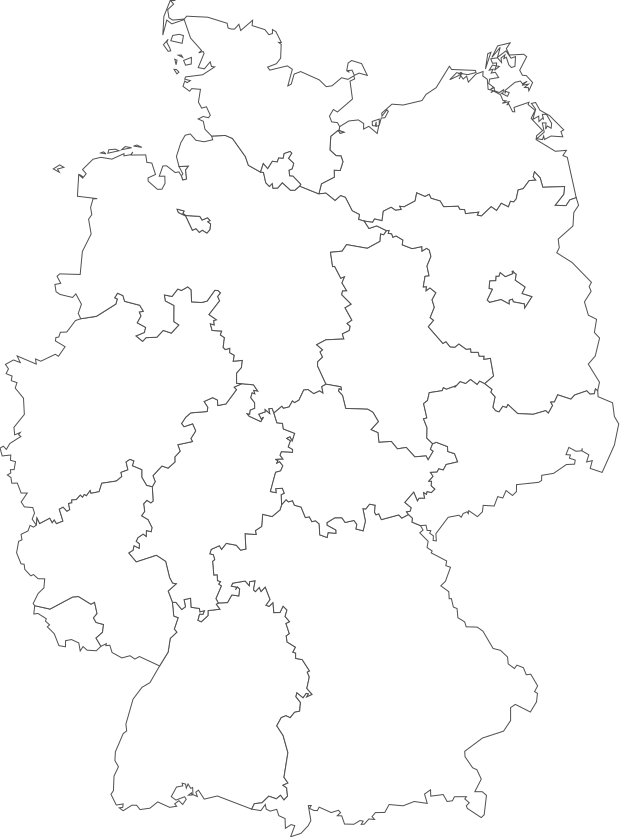
\includegraphics[width=.95\columnwidth]{figures/germany}
	};

	%\draw[help lines,xstep=1,ystep=1] (0,0) grid (8,11);

	\node[draw,thick,fill=green!15] (f1) at (3.5,8) {File 1};
	\node[draw,thick,fill=green!15] (f2) at (6,6.5) {File 2 \& 3};

	\draw[-{Latex[length=3mm]},thick] (f1) -- (f2);

	\node[draw,thick,fill=red!15] at (4.5,2.5) {File 4};
\end{tikzpicture}
